\documentclass[laboratorio]{guia}

\renewcommand{\practicaname}{Apunte}
\def \practnum {1} 
\def \practica {Determinaci\'on de la diferencia de fase entre dos se\~nales}

\def \materia {Laboratorio de F\'\i sica II para Qu\'\i micos}
\def \periodo {2do. Cuatrimestre de 2015}
\def \catedra {Pablo Cobelli}
\def \website {http://materias.df.uba.ar/f2qa2015c2}
 
\usepackage{graphics}
\usepackage{amsmath}
\usepackage{amsfonts}
\usepackage{graphicx}
\usepackage{float}
\usepackage{wrapfig}
\usepackage{subfigure}
\usepackage{bm}
\usepackage{grffile}
\usepackage{color}
\usepackage{framed}
\usepackage[utf8]{inputenc}
\usepackage[T1]{fontenc}
\usepackage{lmodern}
\usepackage{circuitikz}
\usepackage[spanish]{babel}
\usepackage{babelbib}
\selectbiblanguage{spanish}

 

%----------------------------------------------------------
% Agrega al path de figuras el subdirectorio con el mismo
%     nombre que el archivo principal del proyecto
\graphicspath{{./\jobname/}}

%----------------------------------------------------------
% Definicion del entorno 'sabermas'
\makeatletter
\definecolor{shadecolor}{rgb}{0.89,0.91,0.94}
\newenvironment{sabermas}[1]{%
\vfill
\begin{shaded}
  \begin{center}
  {\textsection{Para saber m\'as}}
  \end{center}
  #1
\sf } 
{%
\end{shaded}%
}
\makeatother

%----------------------------------------------------------
% Definicion del entorno 'problema'
\newcounter{ContadorProblema}
\setcounter{ContadorProblema}{0}
\newcounter{TieneFiguraAsociada}
\setcounter{TieneFiguraAsociada}{0}
\newcounter{UbicacionFigura}
\setcounter{UbicacionFigura}{0}

\newenvironment{problema}[2][]
{%
    \ifx\relax#1\relax%
        \setcounter{TieneFiguraAsociada}{0}
        \else
        \setcounter{TieneFiguraAsociada}{1}
    \fi
    \def \archivofigura {#1}
    % 
    \refstepcounter{ContadorProblema}
    \noindent%
    \ifnum\value{TieneFiguraAsociada} < 1%
        {\sffamily \bfseries Problema \arabic{ContadorProblema}.}
        %{\sc {#1}}%
        \par\nobreak\par\nobreak%
        \medskip 
    \else
        % Va con figura; resta determinar de que lado.
        \ifnum\value{UbicacionFigura} < 1
            % Poner la figura del lado derecho
            \begin{minipage}{12.25cm}
            {\sffamily \bfseries Problema \arabic{ContadorProblema}.}
            %{\sc {#1}}%
            \par\nobreak\par\nobreak%
            \medskip 
        \else
            % Poner la figura del lado izquierdo
            \begin{minipage}{4.5cm}
                \centering
                \includegraphics[width=4.5cm]{\archivofigura}
                {\footnotesize {\sffamily Esquema asociado al 
                problema \arabic{ContadorProblema}}.}
            \end{minipage}\hfill%
            \begin{minipage}{12.25cm}
                {\sffamily \bfseries Problema \arabic{ContadorProblema}.}
                %{\sc {#1}}%
                \par\nobreak\par\nobreak%
                \medskip 
        \fi
    \fi
}
{%
    \ifnum\value{TieneFiguraAsociada} < 1%
        % \par \bigskip \vskip 0.3cm
    \else
        % Va con figura; resta determinar de que lado.
        \ifnum\value{UbicacionFigura} < 1
            % Poner la figura del lado derecho
            \end{minipage}\hfill%
            \begin{minipage}{4.5cm}
                \centering
                \includegraphics[width=4.5cm]{\archivofigura}
                {\footnotesize {\sffamily Esquema asociado al 
                problema \arabic{ContadorProblema}}.}
            \end{minipage}
        \else
            % Poner la figura del lado izquierdo
            \end{minipage}%
        \fi
    \fi
    \setcounter{TieneFiguraAsociada}{0}
    \par \bigskip \vskip 0.3cm
    % Permutamos el valor de la ubicacion
    \ifnum\value{UbicacionFigura} < 1
        \setcounter{UbicacionFigura}{1}
    \else
        \setcounter{UbicacionFigura}{0}
    \fi
}

%----------------------------------------------------------
% Definicion/Redefinicion de estilos
\renewcommand{\vec}[1]{\ensuremath{\mathbf{#1}}}



\hyphenation{ coe-fi-cien-tes coe-fi-cien-te au-to-va-lor
              au-to-va-lo-res co-rres-pon-der pro-ble-ma 
              cual-quie-ra po-la-ri-za-cio-nes }

\graphicspath{{./Apunte_I_Diferencia_de_Fase/}}

\usepackage{pythontex}

\begin{document} 
\objetivo{Mostrar c\'omo determinar experimentalmente la diferencia de fase
    entre dos se\~nales el\'ectricas empleando un osciloscopio de dos canales. 
    \tematicas{Diferencia de fase, an\'alisis de se\~nales oscilatorias.}} 
\maketitle

\section{C\'omo determinar una diferencia de fase}

Consideremos dos se\~nales unidimensionales arm\'onicas, que asumiremos
provienen de la medici\'on de dos cantidades dependientes del tiempo: $x(t)$ e
$y(t)$. Supongamos que sabemos que ambas se\~nales oscilan temporalmente a una
misma frecuencia, que denominaremos $\omega$, pero con {\it a priori}
diferentes amplitudes y con una diferencia de fase relativa que simbolizaremos
mediante $\phi$. Las expresiones anal\'\i ticas que las describen son entonces:
\begin{align}
    x(t) &= A \sin \left(\omega t\right), \\
    y(t) &= B \sin \left(\omega t + \phi \right).
\end{align}

Si conectamos estas se\~nales de tensi\'on a los canales 1 y 2 de un osciloscopio de doble
traza funcionando en el {\it modo a base de tiempo}, las se\~nales se ver\'an
en la pantalla seg\'un se muestra en la Figura~\ref{fig:1}. 


\begin{pylabcode}
rc('text', usetex=True)
rc('font', family='serif')
rc('font', size=10.0)
rc('legend', fontsize=10.0)
rc('font', weight='normal')
t = linspace(0,1,100)
figure(figsize=(5, 3.5))
w = 2*np.pi
phi = np.pi/6
A = 0.85
x = A*np.sin(w*t)
B = 1.32
y = B*np.sin(w*t+phi)
plot(t,x,'b', label=r'$x(t)$')
plot(t,y,'r:', label=r'$y(t)$', linewidth=2)
plot((np.pi/2/w,np.pi/2/w),(A*np.sin(np.pi/2),0.20),'k:')
plot(((np.pi/2-phi)/w,(np.pi/2-phi)/w),(B*np.sin(np.pi/2),0.20),'k:')
plot((0,1),(0,0),'k')
xlabel('Tiempo [sec]')
ylabel('Voltaje [V]')
legend(loc='upper right')
annotate(r'$\Delta t$', xy=(0.2,0.2), xytext=(0.185,0.2)) 
savefig('./Apunte_I_Diferencia_de_Fase/BaseTemporal.pdf',bbox_inches='tight')
\end{pylabcode}

La diferencia de fase $\phi$ entre ambas se\~nales est\'a relacionada con la
diferencia $\Delta t$ entre dos m\'aximos pr\'oximos de cada una de ellas
mediante:
\begin{equation}
    \phi = 2\pi \frac{\Delta t}{T},
\end{equation}
siendo $T$ el per\'\i odo de las se\~nales, que cumple $\omega T = 2\pi$. A
partir de este dato, una forma de determinar $\phi$ ser\'\i a medir $\Delta t$
y $T$ con suficiente precisi\'on para as\'\i\  poder determinar $\phi$
empleando la \'ultima expresi\'on. 

Ahora bien, si las mismas se\~nales se analizan con un osciloscopio de doble
traza funcionando en el {\it modo XY}, lo que obtendremos es un gr\'afico
similar al que se muestra en la Figura~\ref{fig:2}. Lo que vemos representado
en dicha figura es $y(t)$ en las ordenadas, en funci\'on de $x(t)$ en las
abcisas. De esta representaci\'on resulta una curva que es el lugar
geom\'etrico descripto por las ecuaciones param\'etricas (1) y (2). La curva
que se obtiene -en el caso m\'as general- es una elipse, con ejes que no caen
{\it a priori} alineados con los ejes horizontal y vertical del osciloscopio.

Resulta sencillo observar que de las ecuaciones (1) y (2) que para $t=0$, $x(0)
= 0$ y $y(0)=B \sin(\phi)$. Esto implica entonces que del cociente entre el
valor de $y$ donde la elipse corta al eje vertical y el valor m\'aximo de la
se\~nal $y$, obtenemos el valor del $\sin(\phi)$. Un an\'alisis similar puede
realizarse sobre el eje horizontal.

\begin{pylabcode}
rc('text', usetex=True)
rc('font', family='serif')
rc('font', size=10.0)
rc('legend', fontsize=10.0)
rc('font', weight='normal')
t = linspace(0,1,100)
figure(figsize=(5, 3.5))
w = 2*np.pi
phi = np.pi/6
A = 0.85
x = A*np.sin(w*t)
B = 1.32
y = B*np.sin(w*t+phi)
plot((0,0),(2,-2),'k')
plot((-2,2),(0,0),'k')
plot(x,y,'g')
plot((A,A),(2,0),'b--')
plot((0,2),(B,B),'r--')
xlabel(r'$x(t)$ en Canal 1 [V]')
ylabel(r'$y(t)$ en Canal 2 [V]')
legend(loc='lower right')
xlim(-2,2)
ylim(-2,2)
annotate(r'$A$', xy=(A,0), xytext=(A-0.05,-0.25)) 
annotate(r'$B$', xy=(0,B), xytext=(-0.20,B-0.05)) 
annotate(r'$A \sin(\phi)$', xy=(A*np.sin(phi),0), 
         xytext=(A*np.sin(phi),-1), 
         arrowprops=dict(facecolor='black', shrink=0.2))
annotate(r'$B \sin(\phi)$', xy=(0,B*np.sin(phi)), 
         xytext=(-1,B*np.sin(phi)), 
         arrowprops=dict(facecolor='black', shrink=0.2))
savefig('./Apunte_I_Diferencia_de_Fase/BaseXY.pdf',bbox_inches='tight')
\end{pylabcode}

\begin{figure}[t!]
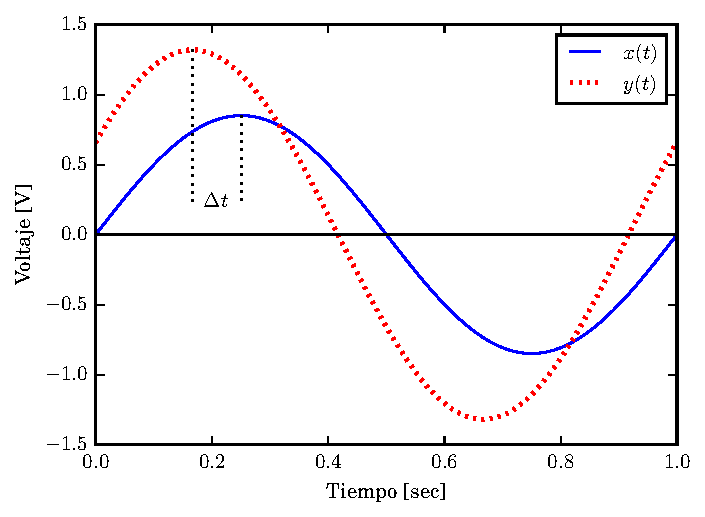
\includegraphics[width=8cm]{BaseTemporal.pdf}
\caption{Representaci\'on de las se\~nales $x(t)$ e $y(t)$ seg\'un se
las observa en un osciloscopio en el {\it modo base de tiempo}.}
\label{fig:1}
\end{figure}
\begin{figure}[t!]
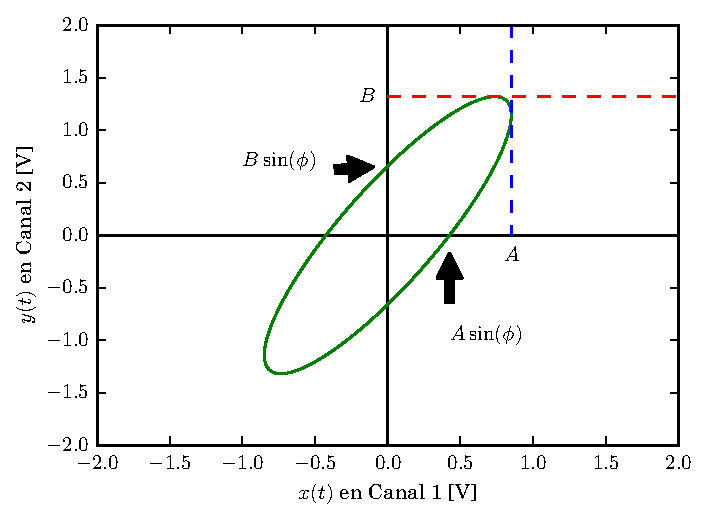
\includegraphics[width=8cm]{BaseXY.pdf}
\caption{Esquema de las se\~nales $x(t)$ e $y(t)$ vistas en el osciloscopio
empleando el {\it modo XY} en el cual pueden observarse las magnitudes de
inter\'es para la determinaci\'on gr\'afica de la diferencia de fase $\phi$.}
\label{fig:2}
\end{figure}

Si las se\~nales se adquieren con un sistema de adquisici\'on de datos asistido
por computadora, recuerde medir las se\~nales $x(t)$ e $y(t)$ por lo menos
durante un per\'\i odo (y con suficiente frecuencia de adquisici\'on), y luego
represente gr\'aficamente $y(x)$ para cada par de puntos obtenido.




% \nocite{Alonso1998,Purcell1988,Reitz1996,Trelles1984}
% \bibliographystyle{unsrt} 
% \bibliography{Bibliografia}

\end{document}
